\documentclass[12pt,english]{article}

\usepackage{amsmath,amssymb,amsthm,epsfig,lineno,rotfloat,psfrag,natbib,caption,setspace,url,bm,geometry}
\usepackage{ecology,algorithm,algorithmic}

\geometry{verbose,letterpaper,tmargin=2.54cm,bmargin=2.54cm,lmargin=2.54cm,rmargin=2.54cm}

%\setlength{\evensidemargin}{0in} \setlength{\oddsidemargin}{0in}
%\setlength{\topmargin}{-0.65in} \setlength{\textwidth}{6.5in}
%\setlength{\textheight}{9.5in} \setlength{\topskip}{0in}
%\setlength{\headheight}{0in}

\bibpunct{(}{)}{,}{a}{}{;}

%\renewcommand{\includegraphics}[2][]{}

\bibliographystyle{ecology}
\raggedbottom


\captionsetup[table]{margin=0pt,font=small,labelfont={sc},justification=justified,labelsep=period}
\captionsetup[figure]{margin=0pt,font=small,labelfont={sc},justification=justified,labelsep=period,name=Fig}



\begin{document}
\begin{spacing}{1.9}


\begin{center}
A guide to Bayesian model checking for ecologists
\bigskip\\
\normalsize
{\sc Paul B. Conn$^{1,}$\footnotemark[5], Mevin B. Hooten$^{2,3,4}$,
Devin S. Johnson$^1$, and Peter L. Boveng$^1$}\smallskip\\
$^1${\em National Marine Mammal Laboratory, NOAA, National Marine Fisheries Service,
Alaska Fisheries Science Center, 7600 Sand Point Way NE, Seattle,
WA 98115 USA }\\ \medskip
$^2${\em U.S. Geological Survey, Colorado Cooperative Fish and Wildlife Research Unit, Colorado State University, Fort Collins, CO 80523 USA }\\ \medskip
$^3${\em Department of Fish, Wildlife, and Conservation Biology, Colorado State University, Fort Collins, CO 80523 USA }\\ \medskip
$^4${\em Department of Statistics, Colorado State University, Fort Collins, CO 80523 USA }\\ \medskip
\end{center}
\footnotetext[5]{Email: paul.conn@noaa.gov}


\raggedright \setlength{\parindent}{0.3in}
%\renewcommand{\baselinestretch}{1.8}\normalsize
\clubpenalty=0

\linenumbers

{\em Abstract.\ }  Checking that models adequately represent data an essential component of applied statistical inference.  Ecologists increasingly use hierarchical, Bayesian statistical models in their research.  The appeal of this modeling paradigm is undeniable, as researchers can build and fit models that embody complex ecological processes while simultaneously controlling for potential biases arising from sampling artifacts. However, ecologists tend to be less focused on checking model assumptions and assessing potential lack-of-fit when applying Bayesian methods than when they apply frequentist methods such as maximum likelihood.  There are also multiple ways of assessing goodness-of-fit for Bayesian models, each of which has strengths and weaknesses.  For instance, in ecological applications, the ``Bayesian p-value" is probably the most widely used approach for assessing lack of fit. Such p-values are relatively easy to compute, but they are well known to be conservative, producing p-values biased towards 0.5.  Alternatively, lesser known approaches to model checking, such as prior predictive checks, probability integral transforms, and pivot discrepancy measures may produce more accurate characterizations of goodness-of-fit but are not as well known to ecologists.  In addition, a suite of visual and targeted diagnostics can be used to examine violations of different model assumptions and lack-of-fit at different levels of the modeling hierarchy, and to check for residual temporal or spatial autocorrelation.  In this review, we synthesize existing literature in order to guide ecologists to the many available options for Bayesian model checking.  We illustrate methods and procedures with several ecological case studies, including i) explaining variation in spatio-temporal counts of bearded seals in the eastern Bering Sea, (ii) modeling the distribution of a herbaceous plant in in the Ozark Highlands of Missouri (USA), and (iii) using resource selection functions to model habitat preferences of XXX.  We argue that model checking is an essential component of scientific discovery and learning that should accompany Bayesian analyses whenever they are used to analyze ecological datasets.


{\em Bayesian p-value, Bayesian qq-plot, count data, goodness-of-fit diagnostic check, hierarchical model, model checking, occupancy, resource selection, pivot discrepancy, predictive distribution, probability interval transform, resource selection, spatio-temporal model}



\def\VAR{{\rm Var}\,}
\def\COV{{\rm Cov}\,}
\def\Prob{{\rm P}\,}
\def\bfX{{\bf X}\,}
\def\bfY{{\bf Y}\,}
\def\bfy{{\bf y}}
\def\bfZ{{\bf Z}\,}
\def\bftheta{\boldsymbol{\theta}}
\def\bfeta{\boldsymbol{\eta}}


\section{Introduction}

Ecologists increasingly use Bayesian methods to analyze complex hierarchical models for natural systems \citep{HobbsHooten2015}.  Adoption of a Bayesian perspective requires that one specify prior distributions for model parameters, a process some have criticized for introducing unneeded subjectivity into the scientific process \citep{LeleDennis2009}.  However, there are clear advantages of adopting a Bayesian mode of inference.  For instance, one can entertain models that were previously intractable using common modes of frequentist statistical inference (e.g., maximum likelihood). Ecologists are using Bayesian modes of inference to fit richer classes of models to their datasets, allowing them to model features such as temporal or spatial autocorrelation, individual level random effects, hidden states, and to separate the effects of process and measurement error \citep{LinkEtAl2002,ClarkBjornstad2004,CressieEtAl2009}. Applying Bayesian calculus also results in posterior probability distributions for parameters of interest; used together with posterior model probabilities, these can provide the basis for mathematically coherent decision and risk analyses \citep{LinkBarker2006,Berger2013}.

Ultimately, the reliability of inferences from a fitted model (Bayesian or otherwise) are dependent on how well the model approximates reality.  There are multiple ways of assessing a model's performance in representing the system being studied. A first step is often to examine diagnostics that compare observed data to model output to pinpoint if and where any systematic differences occur. This process, which we term \textit{model checking}, is an integral part of statistical inference, as it helps diagnose assumption violations and illuminate places where a model might be amended to more faithfully represent gathered data. Following this step, one might proceed to compare the performance of alternative models embodying different hypotheses using any number of model comparison or out-of-sample predictive performance metrics \citep[see][for a review]{HootenHobbs2015} to gauge the support for alternative hypotheses or optimize predictive ability (Fig. \ref{fig:decision}).  Note that scientific inference can still proceed if models do not fit the data well, but conclusions need to be tempered; one approach in such situations is to estimate a variance inflation factor to adjust precision levels downward \citep[e.g.][]{CoxSnell1989,McCullaghNelder1989}.

Non-Bayesian statistical software often include a suite of goodness-of-fit diagnostics that allow practitioners to assess how well different models fit their data.  For instance, when fitting generalized linear \citep{McCullaghNelder1989} or additive \citep{Wood2006} models in the R programming environment \citep{RTeam2013}, one can easily access diagnostics such as quantile-quantile, residual, and leverage plots.  These diagnostics allow one to assess the reasonability of the assumed probability model, to examine whether there is evidence of heteroskedasticity, and to pinpoint outliers.  Likewise, in capture-recapture analysis, there are established procedures for assessing overall fit as well as departures from specific model assumptions which are codified in user-friendly software such as U-CARE \citep{ChoquetEtAl2009}.  Results of such goodness-of-fit tests are routinely reported when publishing analyses in the ecological literature.

The implicit requirement that one conduct model checking exercises is not often adhered to when reporting results of Bayesian analyses in the ecological literature.  For instance, a search of recent volumes of Ecology indicated that only 25\% of articles employing Bayesian analysis on real datasets reported any model checking or goodness-of-fit testing (Fig. \ref{fig:WOS}).  We can think of several reasons why this might be the case.  First, it likely has to do with momentum; the lack of precedent in ecological literature may lead some authors looking for templates on how to publish Bayesian analyses to conclude that model checking is unnecessary.  Second, when researchers seek to publish new statistical methods, applications may be presented more as proof-of-concept exhibits than as definitive analyses that can stand up to scrutiny on their own. In such studies \citep[and textbooks; see e.g.,][]{RoyleDorazio2008}, topics like goodness-of-fit and model checking are often reserved for future research, presumably in journals with less impact .  We (the authors) are certainly culpable of presenting our research in this fashion.  Third, all of the articles we examined did a commendable job in reporting convergence diagnostics to support their contention that Markov chains from MCMC runs had reached their stationary distribution.  Perhaps there is a mistaken belief among authors and reviewers that convergence to a stationary distribution, combined with a lack of prior sensitivity, implies that a model fits the data?  Finally, it may just be that those publishing Bayesian analyses in ecological literature ``. . . like artists, have the bad habit of falling in love with their models" (to borrow a quote attributed to G.E.P. Box and referenced by \citet{LinkBarker2010} with regard to model checking).  We are certainly guilty of this fault as well; indeed this monograph can be viewed as a partial atonement for unrequited love.

If we accept the premise that Bayesian models in ecology should be routinely checked for compatibility with data, a logical next question is how best to conduct such checks.  Unfortunately, there is no single best answer.  Most texts in ecology \citep[e.g.,][]{KingEtAl2009,LinkBarker2010,KerySchaub2012} focus on posterior predictive checks, as pioneered by \citet{Guttman1967}, Rubin (\citeyear{Rubin1981,Rubin1984}), and \citet{GelmanEtAl1996} (among others).  These procedures are also the main focus of popular Bayesian analysis texts \citep[e.g.,][]{CressieWikle2011,GelmanEtAl2014} and are based on the intuitive notion that data simulated from the posterior distribution should be similar to the data one is analyzing.  However, ``Bayesian p-values" generated from these tests tend to be conservative (biased towards 0.5) because the data are in effect used twice \citep[once to fit the model and once to test the model;][]{BayarriBerger2000,RobinsEtAl2000}.  By contrast, other approaches less familiar to ecologists (such as prior predictive checks, probability integral transforms, and pivot discrepancy measures) may produce more accurate characterizations of goodness-of-fit but may require extra data for out-of-sample prediction or may be more difficult to implement.

In this monograph, we have collated relevant statistical literature with the goal of providing ecologists with a practical guide to Bayesian model checking.  We start by defining a consistent notation that we use throughout the paper. Next, we work to compile a bestiary of Bayesian model checking procedures, providing positives and negatives associated with each approach.  After describing several ways in which model checking results can sometimes be misleading (as with hierarchically centered models), we illustrate Bayesian model checking using three case studies.  These include a species distribution model (SDM) developed from bearded seal counts (\textit{Erignathus barbatus}) in the Chukchi Sea, an SDM developed from presence-absence data of a herbaceous plant (\textit{Genus species}) in Missouri, and analysis of animal telemetry data.  We conclude with several recommendations on how model checking results should be presented in the ecological literature.



\section{Background and notation}

Before describing specific model checking procedures, we first establish common notation.  Bayesian inference seeks to describe the posterior distribution, $[\boldsymbol{\theta} | {\bf y}]$, of model parameters, $\boldsymbol{\theta}$, given data, \textbf{y}.  Here and throughout the paper, we use bold lowercase symbols to denote vectors.  Matrices will be represented with bold, uppercase symbols, while roman (unbolded) characters will be used for scalars.  The bracket notation $[ \hdots ]$ denotes a probability distribution or mass function, and a bracket with a vertical bar `$|$' denotes that it is a conditional probability distribution.

The posterior distribution is often written as
\begin{eqnarray}
  [\boldsymbol{\theta} | \textbf{y}] & = & \frac{[\textbf{y} | \boldsymbol{\theta}] [\boldsymbol{\theta}]}{[\textbf{y}]},
\end{eqnarray}
where $[\textbf{y}|\boldsymbol{\theta}]$ is the assumed probability model for the data, given parameters (i.e., the likelihood), $[\boldsymbol{\theta}]$ denotes the joint prior distribution for parameters, and $[\textbf{y}]$ is the marginal distribution of the data.  In Bayesian computation, the denominator $[\textbf{y}]$ is frequently ignored because it is a fixed constant that does not affect inference \citep[although it is needed when computing Bayes factors for model comparison and averaging;][]{LinkBarker2006}.
The exact mechanics of Bayesian inference are well reviewed elsewhere \citep[e.g.,][]{KingEtAl2009,LinkBarker2010,HobbsHooten2015}, and we do not attempt to provide a detailed description here.  For the remainder of this treatment, we assume that the reader has familiarity with the basics of Bayesian inference, including Markov chain Monte Carlo (MCMC) as a versatile tool for sampling from $[\boldsymbol{\theta}|\textbf{y}]$.

In describing different model checking procedures, we will often need to reference data simulated under an assumed model.  We use $\textbf{y}_i^{rep}$ to denote a single, simulated dataset under the model that is being checked.  In some situations, we may indicate that the dataset was simulated using a specific parameter vector, $\boldsymbol{\theta}_i$; in this case, denote the simulated dataset as $\textbf{y}_i^{rep}|\boldsymbol{\theta}_i$.  We use the notation $T(\textbf{y},\boldsymbol{\theta})$ to denote a discrepancy function that is dependent upon data and possibly the parameters $\boldsymbol{\theta}$.  For instance, we might compare the the discrepancy $T(\textbf{y},\boldsymbol{\theta})$ calculated with observed data to a distribution obtained by applying $T(\textbf{y}^{rep},\boldsymbol{\theta})$ to multiple replicated data sets.  Examples of candidate discrepancy functions are provided in Table \ref{tab:discrepancy}.

\section{Model checking procedures}

\subsection{Posterior predictive checks}

Posterior predictive checks are the dominant form of Bayesian model checking advanced in statistical texts read by ecologists \citep[e.g.,][]{KingEtAl2009,LinkBarker2010,KerySchaub2012,GelmanEtAl2014}. Although sample size was small ($n=25$), our survey of recent \textit{Ecology} volumes indicated that posterior predictive checks are also the dominant form of Bayesian model checking being reported in ecological literature (if any checking is reported at all; Fig. \ref{fig:WOS}).  Posterior predictive checks are based on the commonsense notion that data simulated under a fitted model should be comparable to the real world data the model was fitted to. If observed data differ from simulated data in a systematic fashion (e.g, excess zeros, increased skew, lower kurtosis), it is good indication that model assumptions are not being met.

Posterior predictive checks can be used to look at differences between observed and simulated data graphically, or can be used to calculate ``Bayesian p-values" (Alg. \ref{alg:posterior}).  Bayesian p-values necessarily involve application of a discrepancy function, $T(\textbf{y},\boldsymbol{\theta})$, for comparing observed and simulated data.  There are several omnibus discrepancy measures that can be employed to examine overall lack-of-fit, and targeted discrepancy measures can be used to look for specific data features that systematically differ between simulated and observed data (Table \ref{tab:discrepancy}).

Posterior predictive checks are straightforward to implement.  Unfortunately, Bayesian p-values based on these checks tend to be conservative in the sense that the distribution of p-values calculated under a null model (i.e., when the data generating model and estimation model are the same) tends to be dome shaped (e.g., Fig. \ref{fig:pval}) instead of the uniform distribution expected of frequentist p-values \citep{RobinsEtAl2000}. This feature arises because data are used twice: once to approximate the posterior distribution and to simulate the reference distribution for the discrepancy measure, and a second time to calculate the tail probability  \citep{BayarriBerger2000}.  As such, the power of posterior predictive Bayesian p-values to detect significant differences in the discrepancy measure is overstated.  Evidently, the degree of conservatism can vary across data, models, and discrepancy functions, making it difficult to interpret or compare Bayesian p-values across models.

Another possible criticism of posterior predictive checks is that they rely solely on properties of simulated and observed data.  Given that a lack of fit is observed, it may be difficult to diagnose where misspecification is occurring within the modeling hierarchy (e.g., poorly specified priors, errant mean structure, underdispersed error distribution, etc.).  Further, a poorly specified mean structure may still result in reasonable fit of the model if the model is made sufficiently flexible through individual-level random effects (see \textit{Avoiding potential traps with model checking}).

These cautions do not imply that posterior predictive checks are completely devoid of value.  Indeed, given that tests are conservative, small (e.g., $<0.05$) or very large (e.g., $>0.95$) p-values are strongly suggestive of lack-of-fit.  Further, graphical displays (see \textit{Graphical techniques}) and targeted discrepancies (Table \ref{tab:discrepancy}) may help pinpoint common assumption violations (e.g., lack of independence, zero inflation, overdispersion).  However, it is less clear how to interpret p-values and discrepancies that are mildly indicative of lack-of-fit (e.g., a p-value of 0.15 or 0.2).
Several researchers have developed approaches for calibrating Bayesian p-values so that they are asymptotically uniform \citep[e.g.,][]{DeyEtAl1998,BayarriBerger1999}. However, these approaches can be computationally intensive and/or difficult to implement (i.e., custom code is required for each unique application).

Some practical suggestions may help to reduce the degree of conservatism of posterior predictive p-values.  \citet{LunnEtAl2013} suggest that the level of conservatism depends on the discrepancy function used; discrepancy functions that are solely a function of simulated and observed data (e.g., proportion of zeros, distribution of quantiles) may be less conservative than those that also depend on model parameters (e.g., summed Pearson residuals).  Similarly, \citet{MarshallSpiegelhalter2003} suggest reducing the impact of the double use of data by iteratively resimulating random effects when generating posterior predictions for each data point (a procedure they term a ``mixed predictive check").  For an example of this latter approach, see \textit{Spatio-temporal bearded seal counts}.



\subsection{Pivotal discrepancy measures}

In addition to overstated power to detect model lack-of-fit, posterior predictive p-values are limited to examining systematic differences between observed data and data simulated under a hypothesized model.  As such, there is little ability to examine lack-of-fit at higher levels of modeling hierarchy.  One approach to conducting goodness-of-fit at multiple levels of the model is to calculate pivotal quantities \citep{Johnson2004,YuanJohnson2012}.  Pivotal quantities are random variables that can be functions of data, parameters, or both, that have known probability distributions that are independent of parameters \citep[see e.g.,][section 9.2.2]{CasellaBerger1990}.  For instance, consider a simple normal (Gaussian) model
\begin{eqnarray*}
  y & \sim & \mathcal{N}(\mu,\sigma^2).
\end{eqnarray*}
Recall from introductory statistics classes that $z = \frac{y-\mu}{\sigma}$ has a standard $f=\mathcal{N}(0,1)$ distribution; thus $z$ is pivotal quantity in that it has a known distribution independent of $\mu$ or $\sigma$.

This suggests a potential strategy for assessing goodness-of-fit; for instance, in a Bayesian regression model
\begin{eqnarray}
  \label{eq:reg}
  {\bf y} & \sim & \mathcal{N}(\textbf{X} \boldsymbol{\beta},\sigma^2),
\end{eqnarray}
where $\textbf{X}$ represents a design matrix and $\boldsymbol{\beta}$ is a vector of regression coefficients, we might keep track of
\begin{eqnarray}
  \label{eq:resid}
  z_{ij} & = & \frac{y_i - \textbf{x}_i \boldsymbol{\beta}_j}{\sigma_j}
\end{eqnarray}
for each of $j \in {1, 2, \hdots, n}$ samples from the posterior distribution (i.e., drawing each $[\boldsymbol{\beta}_j,\sigma_j] \sim [\boldsymbol{\theta}|{\bf y}]$).  Systematic departures of $z_{ij}$ from the theoretical $N(0,1)$ distribution can point to model misspecification.  Note that although we have again focused on the data model in Eq. \ref{eq:reg}, this same approach could be used at higher levels of the modeling hierarchy.

In practice, there are several difficulties with using pivotal quantities as discrepancy measures in Bayesian model checking.  First, the joint distribution of pivotal quantities calculated across $i \in 1,2,\hdots,n$ samples from the posterior distribution are not independent because they depend on the same observed data, $\textbf{y}$ \citep{Johnson2004}.  As with the Bayesian p-value calculated using a posterior predictive check, this latter problem can result in p-values that are conservative.  \citet{YuanJohnson2012} suggest comparing histograms of a pivotal discrepancy function $T(\textbf{y},\boldsymbol{\theta}_i)$ to its theoretical distribution, $f$, to diagnose obvious examples of model misspecification.  If an omnibus Bayesian p-value is desired, a test can be implemented by appealing to limiting distributions of order statistics \citep{Johnson2004}, but these tests tend to have low power to detect lack of fit.

A second problem is that to apply these techniques, one must first define a pivotal quantity and ascertain its reference distribution. To assess normality is relatively straightforward using standardized residuals (e.g., Eq. \ref{eq:resid}), but pivotal quantities are not necessarily available for other distributions (e.g., Poisson).  However, \citet{YuanJohnson2012}, building upon work of \citet{Johnson2004} proposed an algorithm based on cumulative distribution functions (CDFs) that can apply to any distribution, and at any level of a hierarchical model (Alg. \ref{alg:pivot}).  For continuous distributions, this algorithm works by defining a quantity $w_{ij} = g(y_{ij},\boldsymbol{\theta})$ (this can simply be $w_{ij}=y_{ij}$) with a known CDF, $\Theta$.  Then, according to the probability integral transformation, $\Theta({\bf w})$ should be uniformly distributed if the the modeled distribution function is appropriate.  Similarly, for discrete distributions, we can apply a randomization scheme \citep{Smith1985,YuanJohnson2012} to generate what should be continuously distributed uniform variates.  For example, when $y_{ij}$ has integer valued support, we can define
\begin{eqnarray*}
  w_{ij} & = & F(y_{ij}-1|\boldsymbol{\theta}) + u_{ij} f(y_{ij}|\boldsymbol{\theta}),
\end{eqnarray*}
where $u_{ij}$ is a continuosly uniform random deviate on (0,1) and $F()$ and $f()$ are the cumulative mass and probability mass functions associated with $[{\bf y} | \boldsymbol{\theta}]$, respectively.  In this case, $w_{ij}$ will be uniformly and continuously distributed on (0,1) if the assumed distribution is reasonable; deviation from this distribution can point to model misspecification.

Note that while we have written Alg. \ref{alg:pivot} in terms of the data distribution $[{\bf y} | \boldsymbol{\theta}]$, the algorithm can be applied (without loss of generality) to any level of a hierarchical model. Further, Alg. \ref{alg:pivot} can be applied separately to different categories of mean response (e.g., low, medium, or high levels of predicted responses). These advantages are extremely appealing in that one can more thoroughly test distributional assumptions and look for places where lack-of-fit may be occurring, something that can be difficult to do with posterior predictive checks.  We apply Alg. \ref{alg:pivot} to real data in \textit{Examples} and provide R code for applying this approach to generic MCMC data in the R package \texttt{HierarchicalGOF} accompanying this paper (see \textit{Software} for more information).

\subsection{Prior predictive checks}

\citet{Box1980} argued that the hypothetico-deductive process of scientific learning can be embodied through successive rounds of model formulation and testing. According to his view, models are built to represent current theory and an investigator's knowledge of the system under study; data are then collected to evaluate how well the existing theory (i.e., model) matches up with reality.  If necessary, the model under consideration can be amended, and the process repeats itself.

From a Bayesian standpoint, such successive rounds of \textit{estimation} and \textit{criticism} can be embodied through posterior inference and model checking, respectively \citep{Box1980}.
If one views a model, complete with all its set of assumptions and prior beliefs, as a working model of reality, then data simulated under a model should look similar to data gathered in the real world.  This notion can be formalized through a prior predictive check, where replicate data $\bfy^{rep}$ are simulated via
\begin{eqnarray}
   \label{eq:prior}
   \bftheta^{rep} & \sim & [\bftheta] \\
   \bfy^{rep} & \sim & [\bfy|\bftheta^{rep}] \nonumber
\end{eqnarray}
and then compared to observed data $\bfy$ via a discrepancy function (Alg. \ref{alg:prior}).

Unlike posterior predictive checks, p-values from prior predictive checks are uniformly distributed under the null model and have properly stated frequentist properties.  The main problem with this approach is that the models being considered need to have considerable historical investment and proper prior distributions informed by expert opinion or data from previous studies.  In many cases where Bayesian inference is employed, this is simply not the case.  Still, this approach may be useful for hierarchical models that serve as an embodiment of current theory about a study system (e.g., population or ecosystem dynamics models).  Alternatively, a subset of data (test data) can be withheld when fitting a model, and the posterior distribution $[\bftheta|\bfy]$ can be substituted for $[\bftheta]$ in Eq. \ref{eq:prior}.  If used in this manner, prior predictive checks can be viewed as a form of cross validation, a subject we shall examine next.

\subsection{Cross validation tests}

Cross validation consists of leaving out one or more data points, rerunning analysis, and seeing how model predictions match up with actual observations.  It is most often used to examine the relative predictive performance of different models \citep[i.e., for model selection; see e.g.][]{ArlotCelisse2010}.  However, it also possible to use cross validation techniques to examine model fit and diagnose outlier behavior.  The major advantage of conducting tests in this fashion is that there is no duplicate use of data (as with posterior predictive tests or pivotal discrepancy tests).  The major disadvantage is that it can be computationally challenging for complicated hierarchical models.

One approach to checking models using cross validation in the cross-validated probability integral transform (PIT) test, which has long been exploited to examine the adequacy of probabilistic forecasts \citep[e.g.,][]{Dawid1984,Fruiiwirth1996,GneitingEtAl2007,CzadoEtAl2009}. These tests work by simulating data at a set of times or locations, and computing the CDF of the predictions evaluated at the realized data (where realized data are not used to fit the model).  This can be accomplished in a sequential fashion for time series data, or by withholding data (as with leave-one-out cross validation).  In either case, divergence from a Uniform(0,1) distribution is indicative of a model deficiency.  In particular, a U-shape suggests an underdispersed model, a dome shape suggests an overdispersed model, and skew (i.e., mean not centered at 0.5) suggests bias.  \citet{Congdon2014} suggests an algorithm for computing PIT diagnostic histograms for both continuous and discrete data in Bayesian applications (see Alg. \ref{alg:PIT}).


Cross-validation can also be useful for diagnosing outliers in spatial modeling applications.  For instance, \citet{SternCressie2000} and \citet{MarshallSpiegelhalter2003} use Alg. \ref{alg:PIT} to identify regions that have inconsistent behavior relative to the model.  Such outliers can either indicate that the model does not sufficiently explain variation in responses, that there are legitimate ``hot spots" worthy of additional investigation \cite{MarshallSpiegelhalter2003}, or both.

\subsection{Residual tests}

\citet{LunnEtAl2013} suggest several informal tests based on distributions of Pearson and deviance residuals.  These tests are necessarily informal in Bayesian applications, as residuals all depend on $\bftheta$ and are thus not truly independent as required in unbiased application of goodness-of-fit tests.  Nevertheless, several rules of thumb can be used to screen residuals for obvious assumption violations.  For example, standardized Pearson residuals for continuous data,
\begin{eqnarray*}
  r_i & = & \frac{y_i - E(y_i|\bftheta)}{\sqrt{\textrm{Var}(y_i | \bftheta)}},
\end{eqnarray*}
should generally take on values between -2.0 and 2.0.  Values very far out of this range represent outliers.
Similarly, for the Poisson and binomial distributions, an approximate rule of thumb is that the mean saturated deviance should approximately equal sample size for a well fitting model \citep{LunnEtAl2013}.

For time series, spatial, and spatio-temporal models, failure to account for autocorrelation can result in bias and overstated precision \citep{LichsteinEtAl2002}.  For this reason, it is important to look for evidence of residual spatio-temporal autocorrelation in analyses where data have a spatio-temporal index.  There are a variety of metrics to quantify autocorrelation, depending upon the ecological question and types of data available \cite[e.g.][]{PerryEtAl2002}.  For Bayesian regression models, one versatile approach is to compute a posterior density associated with a statistic such as Moran's I \citep{Moran1950} or Getis-Ord G* \citep{GetisOrd1992} on residuals.  For example, calculating Moran's I for each posterior sample $j$ relative to posterior residuals ${\bf Y} - \textrm{E}({\bf Y} | \boldsymbol{\theta}_j)$, a histogram of $I_j$ values can be constructed; substantial overlap with zero suggests little evidence of residual spatial autocorrelation.  As calculation of Moran's I is dependent upon a a pre-specified distance weighting scheme, investigators might simulate a posterior sample of Moran's I at several different choices of weights or neighborhoods to evaluate residual spatial autocorrelation at different scales.  

\subsection{Just build a bigger model!  Tradeoffs between fit and prediction}

cite Ver Hoef musings

\subsection{Graphical techniques}

Thought maybe I'd make this a separate section because these could potentially could be done with posterior or prior predictive checks, or even with PDMs.  Some ideas: q-q plots, maps (for spatial data), residual and binned residual plots \citep{GelmanEtAl2014}.



\subsection{Assessing path structure}

Hierarchical statistical models can be represented using directed, acyclic graphs (DAGs).  Such graphs represent the directed flow of probability through a model, with the assumption that connected nodes are stochastically dependent; unconnected nodes are assumed to be conditionally independent.  In some models, the direction and connectivity among nodes is canonical and self-evident (for example, generalized regression models).  However, in others (e.g., ecosystem models), there may be considerable uncertainty as to the appropriateness of a particular graph structure.  In the latter case, a general assessment of the graph structure should also be a part of model checking exercises.

\citet{Shipley2009} introduced a directional-separation test for assessing the path structure of DAGs.  According to this test, each pair of nodes that are not directly connected constitute an independence claim (possibly conditional on the values of intervening nodes); each such claim can be assessed via a statistical model.  An overall p-value can then be calculated to assess the validity of the overall path structure.

too far afield?
provide algorithm?


\section{Avoiding potential traps with model checking}

Mean structure vs. dispersion - not always obvious where misspecification occurs.

Hierarchical centering

\section{Computing}

\section{Examples}

\subsection{Modeling the distribution of a herbaceous plant}

\subsection{Spatio-temporal bearded seal counts}

\subsection{Resource selection of XXX}

\section{Discussion}


Focus on prior sensitivity, convergence diagnostics and sometimes model comparison (e.g. DIC or cross validation) - not as much focus on GOF.

GOF on most general model, then model selection/comparison/averaging \citep{BurnhamAnderson2004}.


\centerline{\sc Acknowledgments} Funding
for Bering Sea aerial surveys was provided by the U.S. National Oceanic and Atmospheric
Administration and by the U.S. Bureau of Ocean Energy Management (Interagency
Agreement M12PG00017).  The views and conclusions in this article represent the views of the authors and the U.S. Geological Survey but do not necessarily represent findings or policy of the U.S. National Oceanic and Atmospheric Administration.  Any use of trade, firm, or product names is for descriptive purposes only and does not imply endorsement by the U.S. Government.

\renewcommand{\refname}{Literature Cited}
\bibliography{master_bib}


\pagebreak

ALGORITHMS

\begin{algorithm}
\caption{Posterior predictive check algorithm for computing a Bayesian p-value, $P$ using $m$ samples from the posterior distribution.  A selection of discrepancy measures $T(\textbf{y},\boldsymbol{\theta})$ are provided in Table \ref{tab:discrepancy}.}
\label{alg:posterior}
\begin{algorithmic}
\STATE $P \leftarrow 0$
\FOR{$i \in 1:m$}
  \STATE Draw $\boldsymbol{\theta}_i \sim [\boldsymbol{\theta}|{\bf y}]$
  \STATE Draw $\textbf{y}_i^{rep} \sim [\textbf{y} | \boldsymbol{\theta}_i]$ \STATE Calculate $T_i^{rep} = T(\textbf{y}_i^{rep},\boldsymbol{\theta}_i)$
  \STATE Calculate $T_i^{obs} = T(\textbf{y}_i,\boldsymbol{\theta}_i)$
  \IF{$T_i^{obs} < T_i^{rep}$}
    \STATE $P \leftarrow P+1$
  \ENDIF
\ENDFOR
\STATE $P \leftarrow P/m$
\end{algorithmic}
\end{algorithm}

\begin{algorithm}
\caption{Prior predictive check algorithm for computing a Bayesian p-value, $P$ using $m$ samples from the posterior distribution. A selection of discrepancy measures $T(\textbf{y},\boldsymbol{\theta})$ are provided in Table \ref{tab:discrepancy}.}
\label{alg:prior}
\begin{algorithmic}
\STATE $P \leftarrow 0$
\FOR{$i \in 1:m$}
  \STATE Draw $\boldsymbol{\theta}_i \sim [\boldsymbol{\theta}]$
  \STATE Draw $\textbf{y}_i^{rep} \sim [\textbf{y} | \boldsymbol{\theta}_i]$ \STATE Calculate $T_i^{rep} = T(\textbf{y}_i^{rep},\boldsymbol{\theta}_i)$
  \STATE Calculate $T_i^{obs} = T(\textbf{y}_i,\boldsymbol{\theta}_i)$
  \IF{$T_i^{obs} < T_i^{rep}$}
    \STATE $P \leftarrow P+1$
  \ENDIF
\ENDFOR
\STATE $P \leftarrow P/m$
\end{algorithmic}
\end{algorithm}

\begin{algorithm}
\caption{Algorithm for conducting $\chi^2$ discrepancy check to assess the distribution of modeled quantities.  If distributional assumptions are reasonable, the cumulative distribution function associated with modeled quantities should be uniformly distributed (\citep{Johnson2004,YuanJohnson2012}). Note that $n$ denotes sample size and $m$ denotes the number of posterior samples utilized.  This method relies on binning the pivotal quantity ($w_{ij} = g(y_{ij},\boldsymbol{\theta}_i)$ into $K \times L$ bins, where $K$ and $L$ are fixed by the investigator (bins should be chosen to achieve reasonable sample size in each of the $KL$ bin combinations).  We use $\Theta$ to denote the cumulative distribution function for the distribution of the pivotal quantity.  Specific examples of $g()$ and $\Theta$ are provided in the text.  As written, this algorithm assesses the fit of the data distribution $[{\bf y}|\boldsymbol{\theta}$]; however, note that it can be applied to other levels of a hierarchical model.}
\label{alg:pivot}
\begin{algorithmic}
\STATE Set $b_l \leftarrow l/L$ for $l=0,1,\hdots,L$
\STATE Set $O_{ikl} \leftarrow 0 \hspace{2mm} \forall \hspace{2mm} i \in 1:m, k \in 1:K, l \in 1:L$
\STATE Set $n_{ik} \leftarrow 0 \hspace{2mm} \forall \hspace{2mm} i \in 1:m, k \in 1:K$
\FOR{$i \in 1:m$}
  \STATE Draw $\boldsymbol{\theta}_i \sim [\boldsymbol{\theta}|\textbf{y}]$
  \FOR{$j \in 1:n$}
    \STATE $\mu_{ij} \leftarrow \textrm{E}(y_j|\boldsymbol{\theta}_i)$
    \STATE $w_{ij} \leftarrow g(y_{ij},\boldsymbol{\theta}_i)$
    %\STATE $v_{ij} \leftarrow \VAR(y_j|\boldsymbol{\theta}_i)$
    %\STATE $w_{ij} \leftarrow (y_j-\mu_{ij})v_{ij}^{-0.5}$
  \ENDFOR
  \STATE Set $q_0 \leftarrow -\infty, q_{K} \leftarrow \infty$, and $q_h \leftarrow \textrm{quantile}_{h/K*100\%}(\mu_{ij})$ for $h \in 1:(K-1)$ and the quantile is taken over $j \in 1:n$)
  \FOR{$k \in 1:K$}
    \FOR{$j \in 1:n$}
      \IF{$ q_{k-1} \le \mu_{ij} < q_k $}
        \STATE $r_{ij} \leftarrow k$
        \STATE $n_{ik} \leftarrow n_{ik}+1$
      \ENDIF
    \ENDFOR
    \FOR{$l \in 1:L$}
      \IF{$\Theta(w_{ij}) \in (b_{l-1},b_l]$ \& $r_{ij}=k$}
        \STATE $O_{ikl} \leftarrow O_{ikl}+1$
      \ENDIF
    \ENDFOR
    \STATE Set $T_{ik}({\bf y},\bftheta_i) \leftarrow \sum_{l=1}^L \frac{(O_{ikl}-n_{ik}L^{-1})^2}{n_{ik}L^{-1}} $
  \ENDFOR
  \STATE Set $T_i({\bf y},\bftheta_i) \leftarrow \sum_{k=1}^K T_{ik}({\bf y},\bftheta_i)$
\ENDFOR
\STATE Test $T_{ik}({\bf y},\bftheta_i) \sim \chi^2_{L-1}$ for targeted lack-of-fit
\STATE Test $T_{i}({\bf y},\bftheta_i) \sim \chi^2_{K(L-1)}$ for omnibus lack-of-fit
\end{algorithmic}
\end{algorithm}


\begin{algorithm}
\caption{Algorithm for conducting predictive probability integral transform (PIT) checks, as described by e.g. \citet{Fruiiwirth1996}.  This approach requires having ``test" data; here we assume that a ``leave-one-out" procedure is used, although other  approaches are certainly possible (and may be preferable, especially when sample sizes are large).  To this end, we define $\textbf{y}_{-i}$ as the set of data for which the $i$th observation is missing, $m$ to be the total number of observations, and $n$ to be the number of posterior samples that are analyzed for each data set.  The indicator function $I(A)$ takes on the value 1.0 if the statement $A$ is true, and is 0.0 otherwise.}
\label{alg:pivot}
\begin{algorithmic}
\STATE Set $u_j = 0 \forall j \in 1,2,\hdots,n$
\FOR{$i \in 1:m$}
  \FOR{$j \in 1:n$}
    \STATE Simulate a draw $\boldsymbol{\theta}_{ij}$ from the posterior distribution $[\theta | \textbf{y}_{-i}] \propto [ \textbf{y}_{-i} | \theta][\theta]$
    \STATE Simulate a posterior prediction $\tilde{y}_{ij}$ from the predictive density (or mass function), $[y_i | \boldsymbol{\theta}_{ij}]$
  \ENDFOR
    \IF{$y_i$ has continuous support}
      \STATE{Set $u_i = \sum_j I(\tilde{y}_{ij} \le y_i)$}
    \ENDIF
    \IF{$y_i$ has nonnegative integer support (i.e. for count data)}
      \STATE{Set $u_i = \sum_j I(\tilde{y}_{ij} < y_i) + 0.5 I(\tilde{y}_{ij}=y_ij)$}
    \ENDIF
    \IF{$y_i$ has binary support}
      \STATE{Set $u_i = \sum_j I(\tilde{y}_{ij}=y_ij)$}
    \ENDIF
\ENDFOR
\STATE Plot a histogram of $u_i$ values.  Divergence from a Uniform(0,1) distribution is indicative of lack of fit.  Very high or very low values may indicate outliers.
\end{algorithmic}
\end{algorithm}

\pagebreak




TABLES


\begin{table}[ht]
\caption{Discrepancy functions and pivotal quantities useful for hierarchical model checking.
}
\label{tab:discrepancy}
\centering
\begin{tabular}{p{4cm}lp{5cm}}
  \hline
  Name & Definition & Comments \\
  \hline
  \multicolumn{3}{l}{\textbf{A. Omnibus discrepancy functions}} \\
  $\chi^2$ & $T(\textbf{y},\boldsymbol{\theta}) = \sum_i \frac{(y_i - E(y_i|\boldsymbol{\theta}))^2}{\textrm{var}(y_i|\boldsymbol{\theta})}$ & Often used for count data; suggested by \citet{GelmanEtAl2014} (among others).\\
  Deviance ($D$) &  $T(\textbf{y},\boldsymbol{\theta}) = -2 \log [{\bf y} | \boldsymbol{\theta}]$ & used by \citet{KingEtAl2009}\\
  Likelihood ratio statistic & $T(\textbf{y},\boldsymbol{\theta}) = 2 \sum_i y_i \log(\frac{y_i}{E(y_i|\boldsymbol{\theta})})$ & used by \citet{LunnEtAl2013} \\
  Freeman-Tukey Statistic & $T(\textbf{y},\boldsymbol{\theta})=\sum_i (\sqrt{y_i}-\sqrt{\textrm{E}(y_i|\boldsymbol{\theta})})^2$ & Less sensitive to small expected values than $\chi^2$; suggested by \citet{KeryRoyle2016}.\\
  \multicolumn{3}{l}{\textbf{B. Targeted discrepancy functions}} \\
  Proportion of zeros & $T(\textbf{y}) = \sum_i I(y_i = 0) $ & Zero inflation check for count data \\
  Skewness checks & $T(\textbf{y}) = y_{p\%} $ & Using the $p\%$ quantile can be useful for checking for over- or underdispersion. \\
  \multicolumn{3}{l}{\textbf{C. Pivotal quantities}} \\
  $Y  \sim \textrm{Exponential}(\lambda)$ & $\lambda \bar{Y} \sim \textrm{Gamma}(n,n)$ & Note $n$ is sample size\\
  $Y \sim \mathcal{N}(\mu,\sigma^2)$ (Gaussian) & $ \frac{Y - \mu}{\sigma} \sim \mathcal{N}(0,1) $ & For mean $\mu$ and standard deviation $\sigma$  \\
  $Y \sim \textrm{Weibull}(\alpha,\beta)$ & $ \beta Y^\alpha \sim \textrm{Exponential}(1) $ & \\
  $Y$ from {\it any} distribution & $Z = \frac{\bar{Y}-\mu}{\sigma/\sqrt{n}} \xrightarrow[]{\mathcal{D}} \mathcal{N}(0,1)$ & For large sample size ($n$), $Z$ converges in distribution to a standard normal (Slutsky's theorem) and $Z$ is termed an ``asymptotically pivotal quantity." \\
\hline
\end{tabular}
\end{table}


\begin{table}[ht]
\caption{A summary of Bayesian model checking approaches.  For each method, we describe whether each method allows for (1) computation of an overall p-value (``p-value?"), (2) whether the method tends to be conservative (i.e., has overstated power to detect goodness-of-fit; ``conservative?"), (3) whether all levels of the modeling hierarchy can be evaluated (``all levels?"), and (4) whether out-of-sample data are needed to assess lack-of-fit (``out-of-sample?").
}
\label{tab:discrepancy}
\centering
\begin{tabular}{lcccc}
  \hline
  Method & p-value? & conservative? & all levels? & out-of-sample?  \\
  \hline
  Pivotal discrepancy & Yes & Yes & Yes & No \\
  Posterior predictive check & Yes & Yes & No & No \\
  Prior predictive check & Yes & No & No & Yes \\
  Predictive PIT tests & No & No & No & Yes \\
  Graphical & No & Maybe & Yes & No \\
\hline
\end{tabular}
\end{table}
\pagebreak

FIGURE CAPTIONS

FIGURE 1.  A decision diagram describing the steps we suggest ecologists adopt when reporting the results of Bayesian analyses in the literature, particularly when results will be used for conservation and management or to inform ecological theory.  The first step is to formulate reasonable ecological models, ensuring that the model(s) and associated software is free of errors and that convergence to the posterior distribution can be achieved (using Markov chain Monte Carlo, for instance).  Following this step, models should be checked against observed data to diagnose possible model misspecification (the subject of this article).  Assuming no obvious inadequacies, various model comparison or averaging techniques can be used to compare the predictive performance of alternative models that embody different ecological hypotheses.  Finally, we suggest conducting robustness analyses (prior sensitivity analyses, simulation analyses where model assumptions are violated) to gauge the importance of implicit parametric assumptions on ecological inference.

FIGURE 2.  Type of model checking procedures used in $n=31$ articles published in the journal Ecology during 2014 and 2015. Articles were found via a Web of Science for articles including the topic ``Bayesian" (search conducted 10/1/2015).  Six articles were determined to be non-applicable (N/A) because they either (1) were simulation studies, or (2) used approximate Bayesian computation, which is conceptually different than traditional Bayesian inference \citep[see e.g.][]{BeaumontEtAl2002}.  Of the remaining 25, 20 did not report any model checking procedures.  Five articles reported specific model checking procedures, which included a combination of Bayesian cross validation (\textit{Cross.val}, ), frequentist software (\textit{Non-Bayes}), posterior predictive p-values (\textit{Pp.pval}), and posterior predictive graphical checks (\textit{Pp.gc}).  Some articles also investigated prior sensitivity which can be regarded as a form of model checking, but we do not report prior sensitivity checks here.

FIGURE 3.  Summary of 10,000 Bayesian posterior predictive p-values generated using Algorithm \ref{alg:posterior} under a $\chi^2$ discrepancy function.  In each case, $n=10$ counts were generated from a Poisson($\lambda$) distribution where $\lambda \sim \textrm{Uniform}(1,10)$ and Markov chain Monte Carlo was used to fit the correct (Poisson) model to the data.  For an unbiased test, the observed histogram would be approximately uniform.  In this case, the dome shape indicates the test tends to be too conservative (i.e., the probability of making a type I error is smaller than stated and the power of the test is overstated).

\pagebreak

\begin{figure*}
\begin{center}
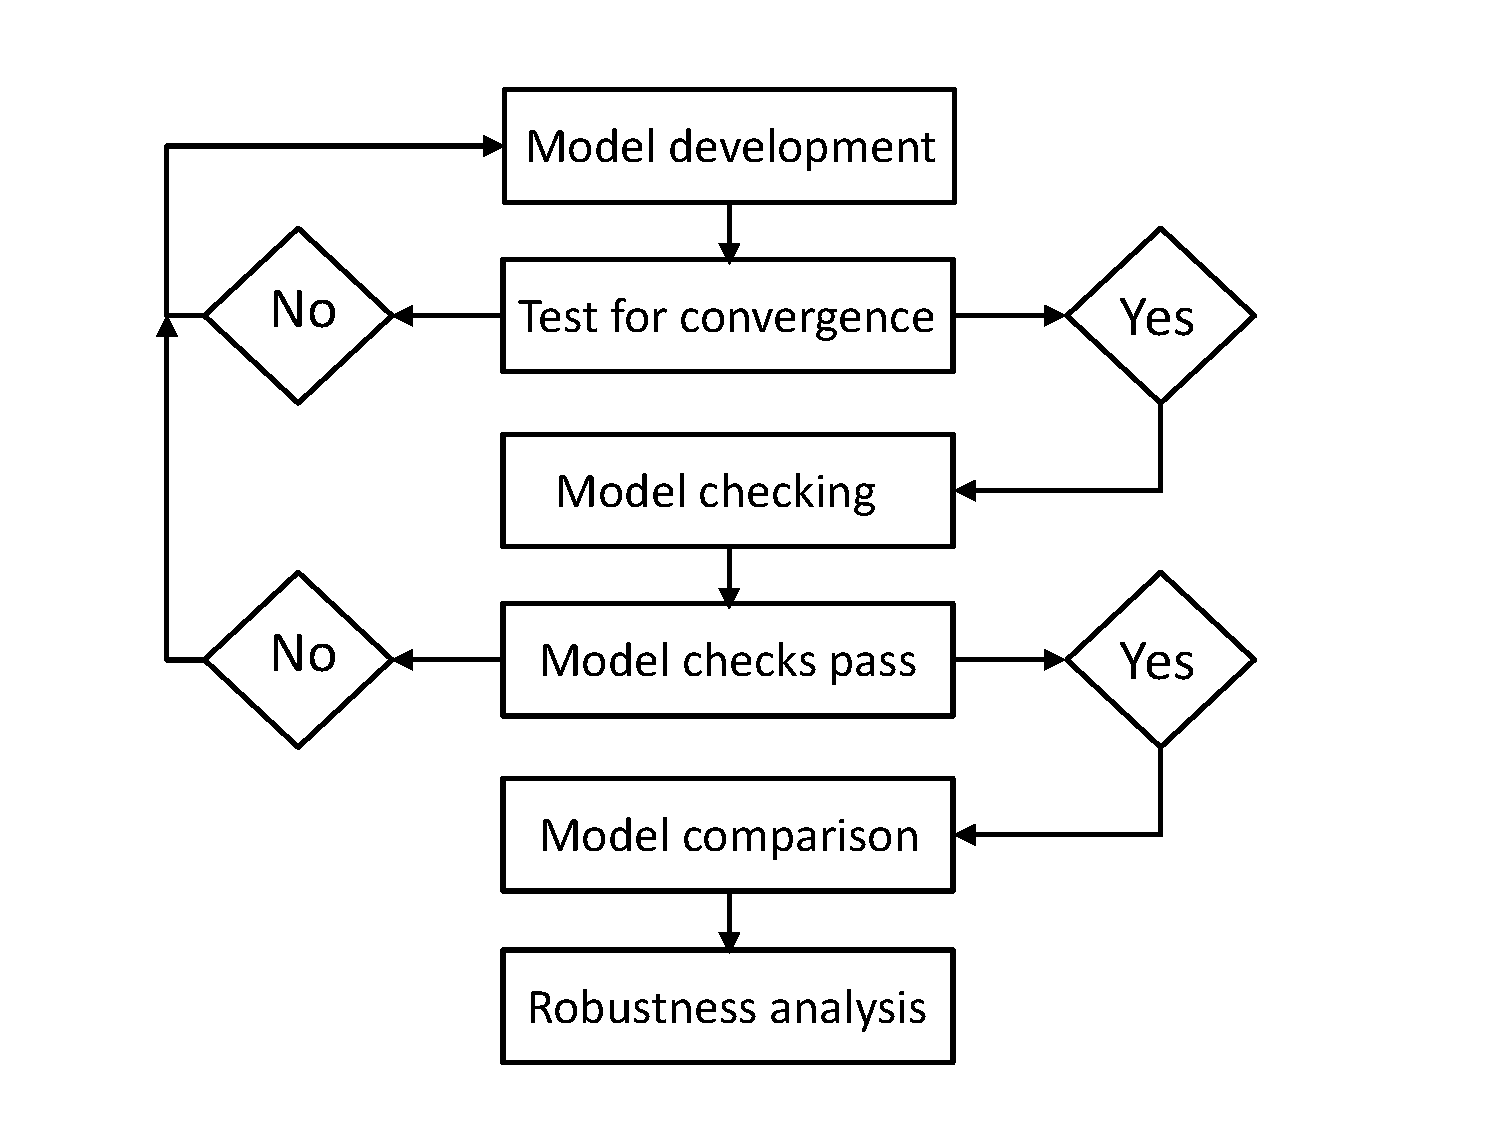
\includegraphics[width=170mm]{Bayesian_modeling_decision_diagram.pdf}
\caption{} \label{fig:decision}
\end{center}
\end{figure*}

\begin{figure*}
\begin{center}
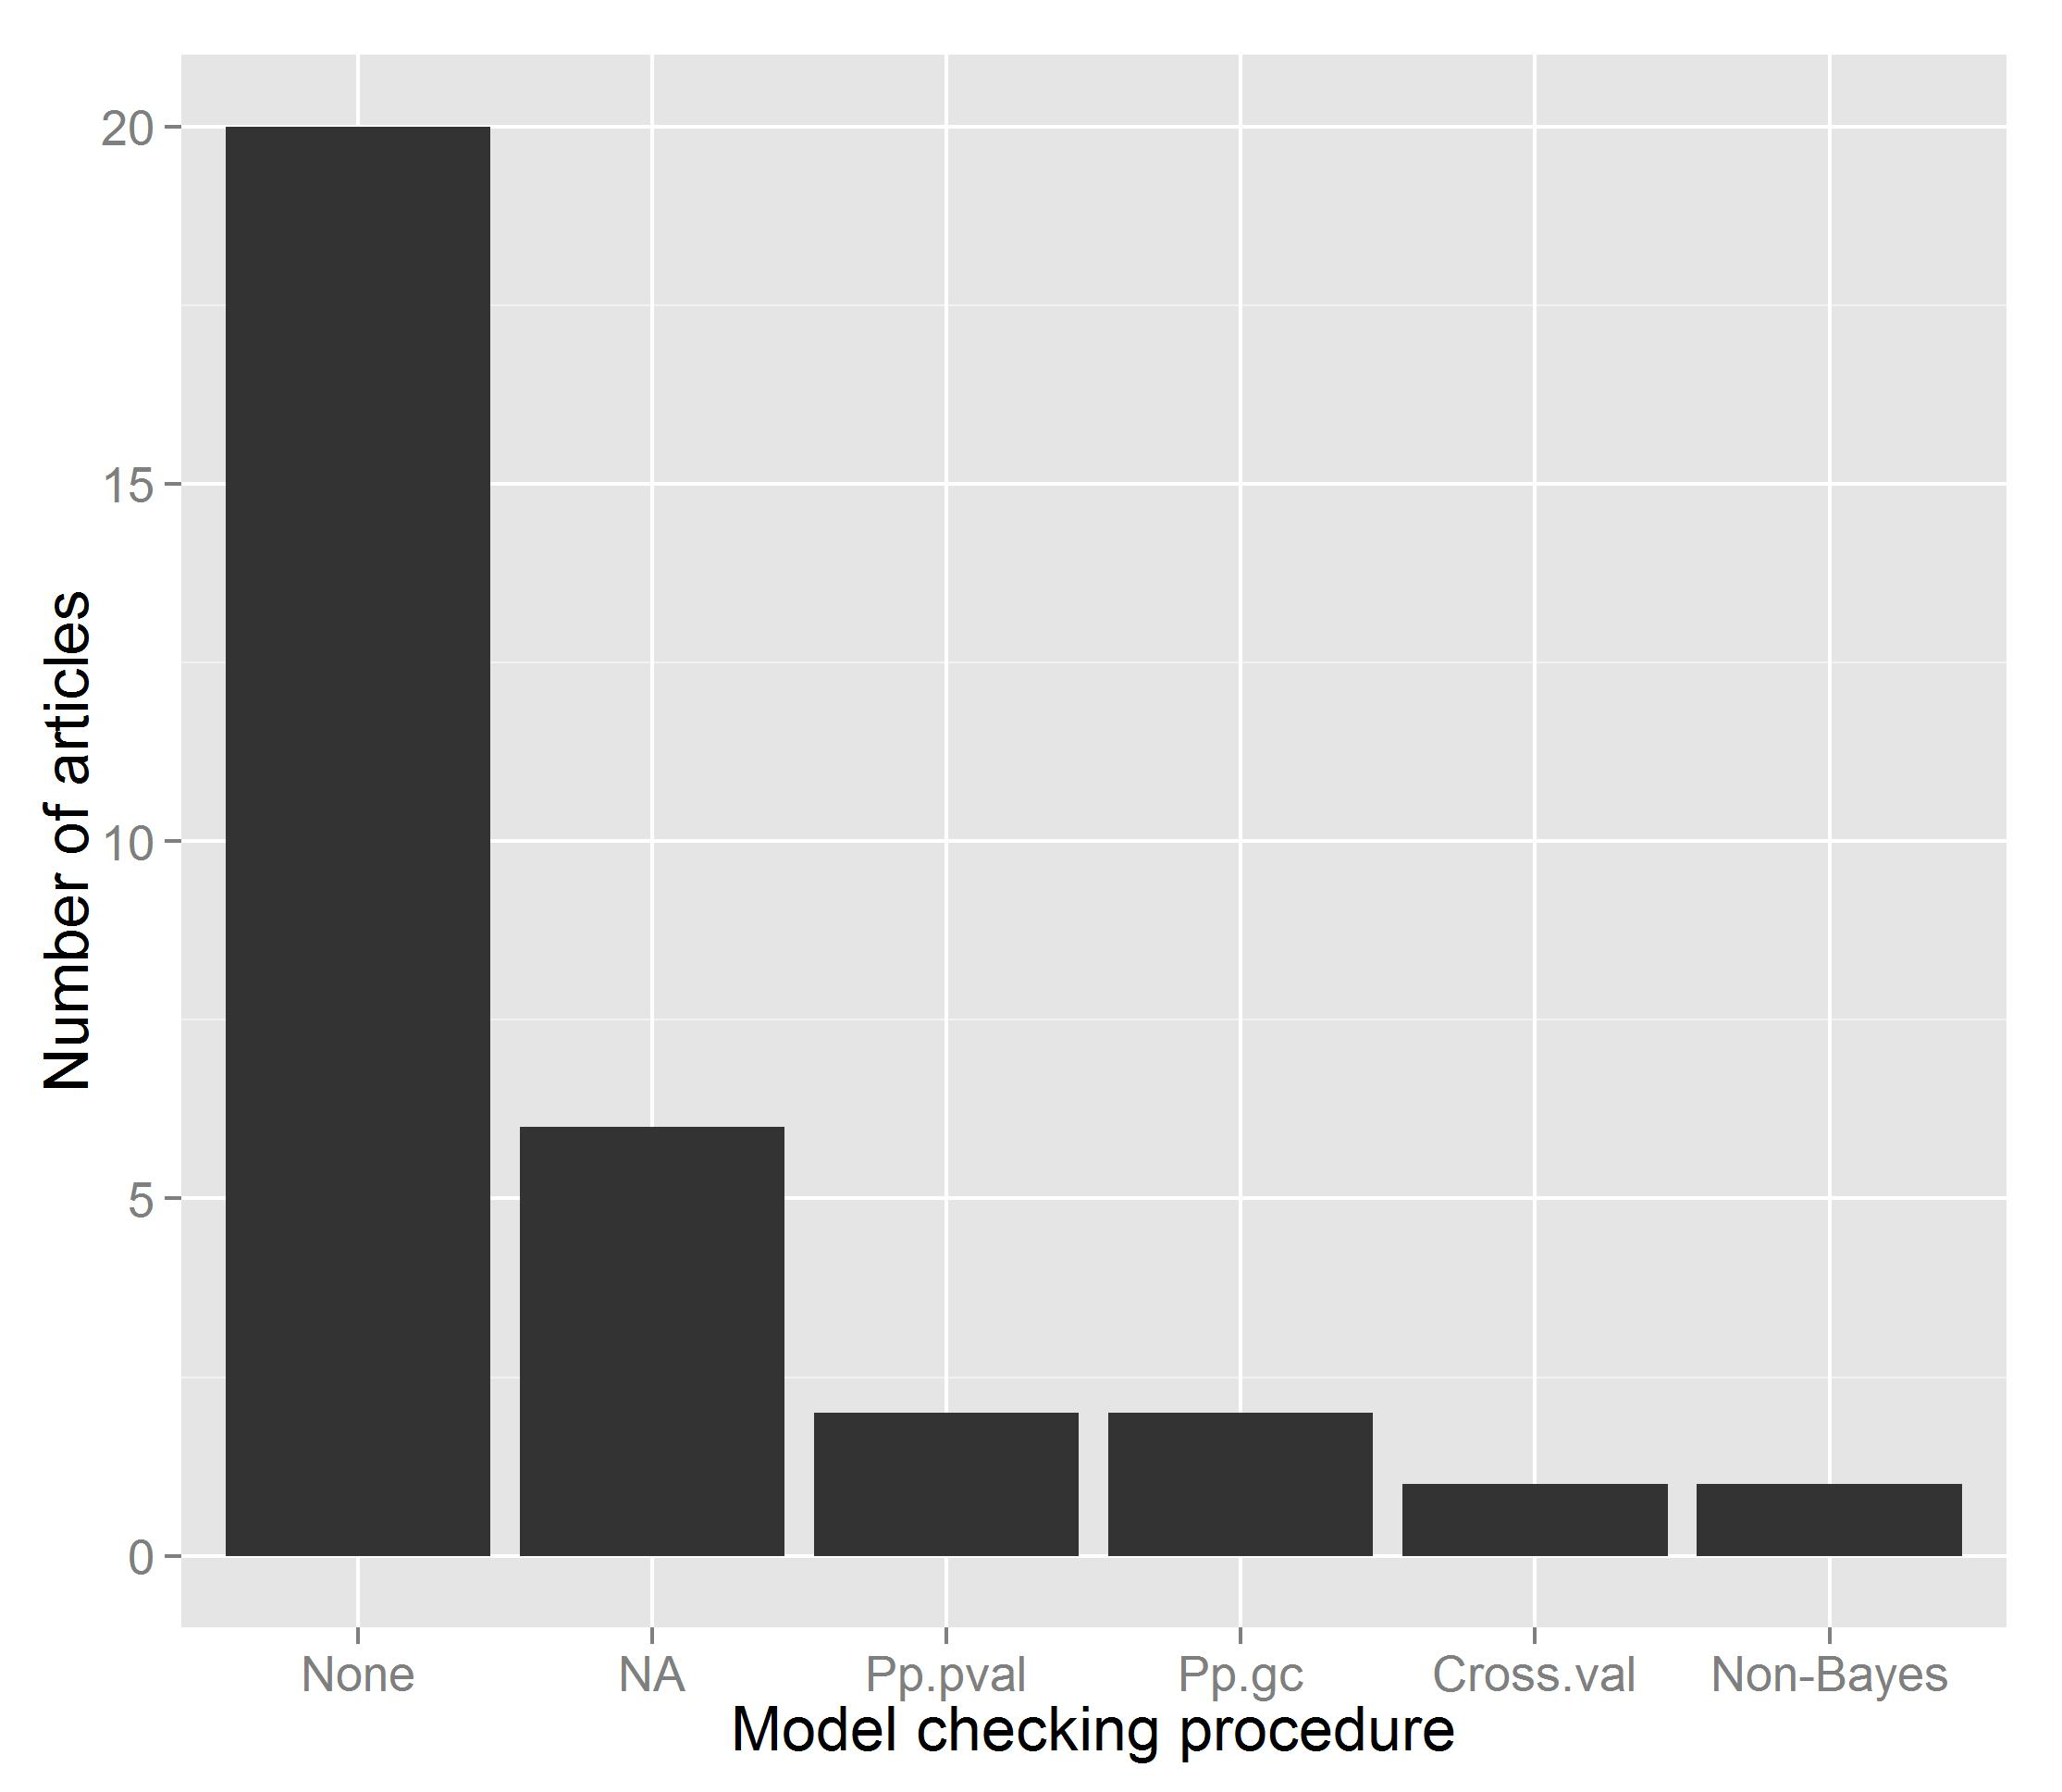
\includegraphics[width=170mm]{WOSsearch.jpeg}
\caption{} \label{fig:WOS}
\end{center}
\end{figure*}

\begin{figure*}
\begin{center}
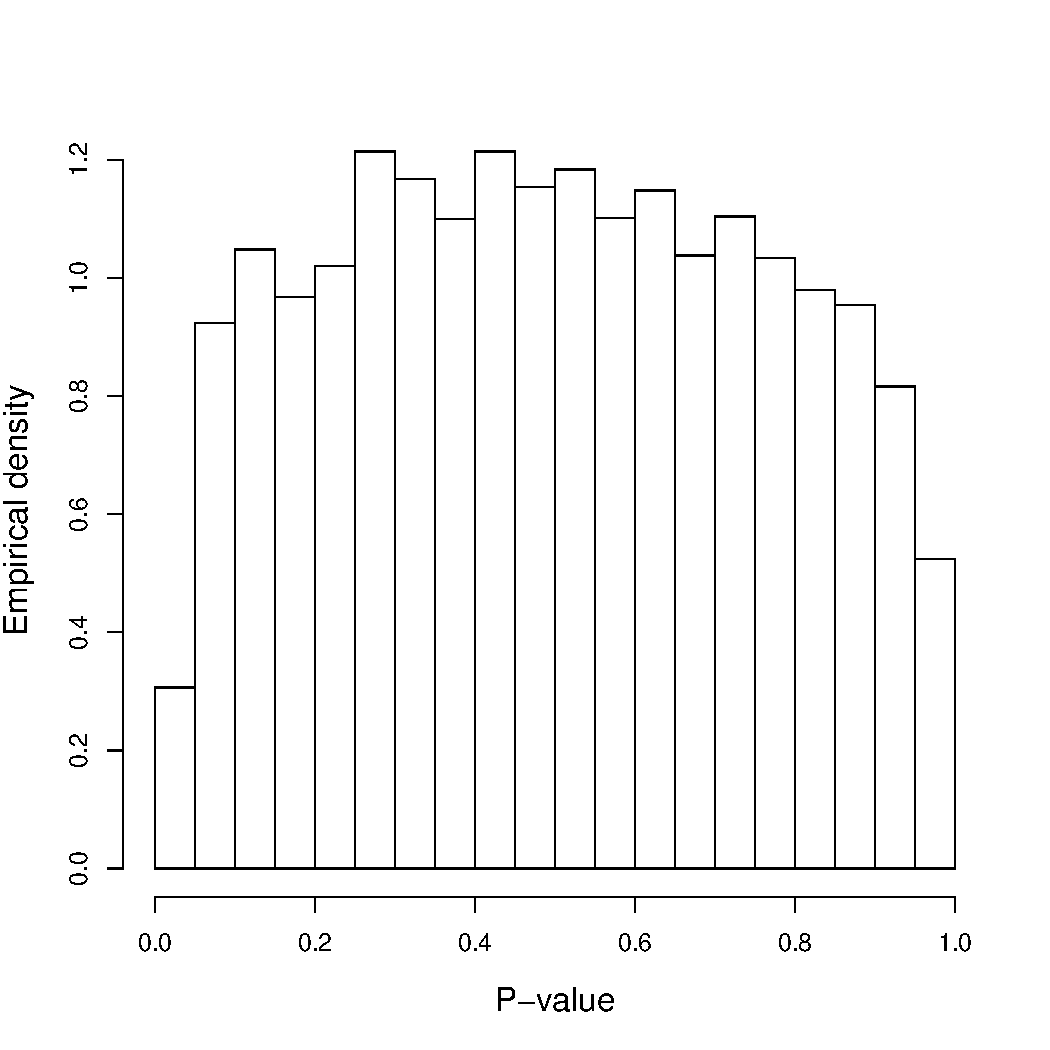
\includegraphics[width=170mm]{Pval_hist.pdf}
\caption{} \label{fig:pval}
\end{center}
\end{figure*}

\end{spacing}
\end{document}
